\documentclass[a3paper, 12pt, landscape]{article}
\usepackage[utf8]{inputenc}
\usepackage[T1]{fontenc}
\usepackage{ngerman, lmodern}
\usepackage[left=1cm, right=1cm, top=2cm, bottom=2cm]{geometry}

\usepackage{color, amsmath, amsthm, caption}
\usepackage{fancyhdr}
  \lhead{}
  \chead{}
  \rhead{\nouppercase\leftmark}
  \lfoot{}
  \cfoot{\thepage}
  \rfoot{}
\usepackage{multicol}
\columnseprule0.4pt
\columnsep1cm

\usepackage{graphicx}
\newenvironment{Figure}
  {\par\medskip\noindent\minipage{\linewidth}}
  {\endminipage\par\medskip}

\newcommand{\TODO}{\textcolor{red}{ \textbf TODO }}
\newcommand{\mathematik}{\begin{equation*}\begin{aligned}}
\newcommand{\mathematikstop}{\end{aligned}\end{equation*}}
\renewcommand{\phi}{\varphi} % make "stroked" phi look "loopy"
\renewcommand{\rho}{\varrho}
\newcommand{\half}{\frac{1}{2}} % 1/2
\newcommand{\phid}{\dot{\phi}}  % phi with one dot
\newcommand{\intend}{\,\mathrm{d}} % end of integral
\newcommand{\EQU}{\qquad\bigg|\,} % separator for explanations for equivalent rearrangements

\title{\fontsize{50pt}{120pt}\selectfont Euler-Lagrange-Gleichungen des Doppelpendels}
\author{ }
\date{ }

\begin{document}

\LARGE
\maketitle

\begin{multicols}{2}

\begin{Figure}
\centering
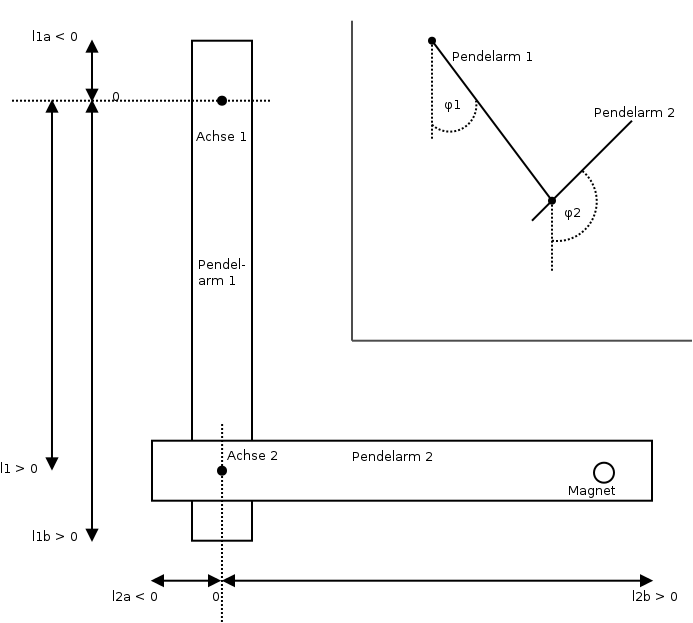
\includegraphics[width=0.8\textwidth]{links_mathsketch_dia.png}
\captionof{figure}{\Large Bedeutung der Variablen}
\end{Figure}
\columnbreak


Ausgangsgleichungen:

\mathematik
\text{Kinetische Energie:} \qquad && T &= \half m \cdot v^2 \\
\text{Geschwindigkeit:} \qquad && v &= \dot{x} + \dot{y} \\
\text{Potentielle Energie:} \qquad && V &= m \cdot g \cdot h \\
\mathematikstop

Position von Massenpunkten $i$ abhängig von Winkeln und Radius $r$ im Intervall $[a; b]$ entlang der Pendel:

\mathematik
&x^{(i)}_1 = r^{(i)} sin \phi_1 \qquad && y^{(i)}_1 = -r^{(i)}_1 cos \phi_1 \\
& x^{(i)}_2 = l_1 sin \phi_1 + r^{(i)}_2 sin \phi_2 && y^{(i)}_2 = -l_1 cos \phi1 - r^{(i)}_2 cos \phi_2
\mathematikstop

Kinetische Energie $T$ und potentielle Energie $V$ des ersten Pendelarms; die Massepunkte werden durch die Dichtefunktion $\rho(r)$ wiedergespiegelt:

\mathematik
T_1 &= \half \int^{l_{1b}}_{l_{1a}} \rho_1(r) \; \left(v_1^{(r)}\right)^2 \intend r \\
    &= \half \int^{l_{1b}}_{l_{1a}} \rho_1(r) \; r^2 \phid_1^2 cos^2 \phi_1 \intend r + \half \int^{l_{1b}}_{l_{1a}} \rho_1(r) \; r^2 \phid_1^2 sin^2 \phi_1 \intend r \\
    &= \half \phid_1^2 \int^{l_{1b}}_{l_{1a}} \rho_1(r) \; r^2 \intend r \\
    &= \half \; \phid_1^2 \; k_1 \\
\textcolor{red}{k_1} &= \int^{l_{1b}}_{l_{1a}} \rho_1(r) \; r^2 \intend r
\mathematikstop

Potentielle Energie des ersten Pendelarms:
\mathematik
V_1 &= \int^{l_{1b}}_{l_{1a}} \rho_1(r) \; y^{(r)}_1 g \\
    &= \int^{l_{1b}}_{l_{1a}} \rho_1(r) \;  (-r) \; cos \phi_1 \cdot g \intend r \\
    &= -g \int^{l_{1b}}_{l_{1a}} \rho_1(r) \; r \; cos \phi_1 \intend r \\
    &= -g \; cos \phi_1 \int^{l_{1b}}_{l_{1a}} \rho_1(r) \; r \intend r \\
    &= -g \; k_2 \; cos \phi_1 \\
\textcolor{red}{k_2} &= \int^{l_{1b}}_{l_{1a}} \rho_1(r) \; r \intend r
\mathematikstop

\columnbreak
Kinetische und potentielle Energie des zweiten Pendelarms:
\mathematik
T_2 &=&& \half \int^{l_{2b}}_{l_{2a}} \rho_2(r)\; \left(v^{(r)}_2\right)^2 \intend r \\
    &=&& \half \int^{l_{2b}}_{l_{2a}} \rho_2(r)\; ( l_1^2 \phid_1^2 + r_2^2 \phid_2^2 \\ &&& + 2 l_1 r_1 \phid_1 \phid_2 (cos \phi_1 \; cos \phi_2 + sin \phi_1 \; sin \phi_2) ) \intend r \\
    &=&& \half \int^{l_{2b}}_{l_{2a}} \rho_2(r)\; l_1^2 \phid_1^2 \intend r + \half \int^{l_{2b}}_{l_{2a}} \rho_2(r) \; r_2^2 \phid_2^2 \intend r \\
    &&&+ \int^{l_{2b}}_{l_{2a}} \rho_2(r) \; l_1 r_2 \phid_1 \phid_2 \; cos(\phi_1 - \phi_2) \intend r \\
    &=&& \half l_1^2 \phid_1^2 \int^{l_{2b}}_{l_{2a}} \rho_2(r) \intend r + \half \phid_2^2 \int^{l_{2b}}_{l_{2a}} \rho_2(r) \; r^2 \intend r \\
    &&&+ l_1 \phid_1 \phid_2 \; cos(\phi_1 - \phi_2) \int^{l_{2b}}_{l_{2a}} \rho_2(r) \; r \intend r \\
    &=&& \half l_1 \phid_1^2 k_3 + \half \phid_2^2 k_4 + l_1 \phid_1 \phid_2 k_5 \; cos(\phi_1 - \phi_2) \\
\textcolor{red}{k_3} &=&& \int^{l_{2b}}_{l_{2a}} \rho_2(r) \intend r \\
\textcolor{red}{k_4} &=&& \int^{l_{2b}}_{l_{2a}} \rho_2(r) \; r^2 \intend r \\
\textcolor{red}{k_5} &=&& \int^{l_{2b}}_{l_{2a}} \rho_2(r) \; r \intend r
\mathematikstop
\mathematik
V_2 &= \int^{l_{2b}}_{l_{2a}} \rho_2(r) \; (-l_1 cos \phi_1 - r\; cos \phi_2) g \intend r\\
    &= - \int^{l_{2b}}_{l_{2a}} \rho_2(r) \; g \; l_1 \; cos\phi_1 \intend r - \int^{l_{2b}}_{l_{2a}} \rho_2(r)\; g\; r \; cos \phi_2 \intend r\\
    &= -g\;l_1\;cos \phi_1 \int^{l_{2b}}_{l_{2a}} \rho_2(r) \intend r - g\; cos \phi_2 \int^{l_{2b}}_{l_{2a}} \rho_2(r) \; r \intend r\\
    &= -g\; l_1\; k_3\; cos \phi_1 - g\; k_5\; cos \phi_2
\mathematikstop

Lagrange-Gleichung:
\mathematik
L &= &&(T_1 + T_2) - (V_1 + V_2) = T_1 + T_2 - V_1 - V_2\\
  &= &&\half \phid_1^2 k_1 + \half l_1 \phid_1^2 k_3 + \half \phid_2^2 k_4 + l_1 \phid_1 \phid_2 k_5 cos(\phi_1 - \phi_2)\\
  &  &&+ g k_2 cos \phi_1 + g l_1 k_3 cos \phi_1 + g k_5 cos \phi_2
\mathematikstop

Lagrange-Formalismus für jede der beiden generalisierten Koordinaten:

\mathematik
\dot{p}_1 - \frac{\partial L}{\partial \phi_1} &= 0 \qquad &\text{mit}\quad && p_1 = \frac{\partial L}{\partial \phid_1} \\
\dot{p}_2 - \frac{\partial L}{\partial \phi_2} &= 0        &\text{mit}\quad && p_2 = \frac{\partial L}{\partial \phid_2}\\
\mathematikstop

Umformungen für den generalisierten Impuls $p$:

\mathematik
p_1 &=&& \phid_1 k_1 + l_1 \phid_1 k_3 + l_1 \phid_2 k_5 cos(\phi_1 - \phi_2)\\
0 &=&& \dot{p}_1 - \frac{\partial L}{\partial \phi_1} \\
  &=&& \dot{p}_1 - (-l_1 \phid_1 \phid_2 k_5 sin(\phi_1 - \phi_2) \\ &&& - g k_2 sin \phi_1 - g l_1 k_3 sin \phi_1)\\
\mathematikstop
\mathematik
\textcolor{red}{\dot{p}_1} & \textcolor{red}{= -l_1 \phid_1 \phid_2 k_5 sin(\phi_1 - \phi_2) - g k_2 sin \phi_1 - g l_1 k_3 sin \phi_1}
\mathematikstop

Generalisierter Impuls des zweiten Pendelarms:

\mathematik
p_2 &= \phid_2 k_4 + l_1 \phid_1 k_5 + cos(\phi_1 - \phi_2)\\
0 = \dot{p}_2 - \frac{\partial L}{\partial \phi_2} &= \dot{p}_2 - (l_1 \phid_1 \phid_2 k_5 sin(\phi_1 - \phi_2) - g k_5 sin \phi_2)\\
\textcolor{red}{\dot{p}_2} & \textcolor{red}{= l_1 \phid_1 \phid_2 k_5 sin(\phi_1 - \phi_2) - g k_5 sin \phi_2}
\mathematikstop

Nach dem simultanen Umformen von $p_1$ und $p_2$ zu den Winkelgeschwindigkeiten:

\mathematik
\textcolor{red}{\phid_1} & \textcolor{red}{= \frac{k_4 p_1 - k_5 l_1 p_2 sin(\phi_1 - \phi_2)}{k_1 k_4 + l_1 (k_3 k_4 - k_5^2 l_1 sin(\phi_1 - \phi_2) cos(\phi_1 - \phi_2)}}\\
\textcolor{red}{\phid_2} & \textcolor{red}{= \frac{k_1 p_2 + l_1 (k_3 p_2 - k_5 p_1 cos(\phi_1 - \phi_2))}{k_1 k_4 + l_1 (k_3 k_4 - k_5^2 sin(\phi_1 - \phi_2) cos(\phi_1 - \phi_2)}}
\mathematikstop

Die rot markierten Gleichungen ergeben das für eine Simulation wichtige Differentialgleichungssystem:

\mathematik
\phid_1 &= \frac{k_4 p_1 - k_5 l_1 p_2 cos(\phi_1 - \phi_2)}{k_1 k_4 + l_1 \cdot (k_3 k_4 - k_5^2 l_1 cos^2(\phi_1 - \phi_2))} \\[0.5\baselineskip]
\phid_2 &= \frac{k_1 p_2 + l_1 \cdot (k_3 p_2 - k_5 p_1 cos(\phi_1 - \phi_2))}{k_1 k_4 + l_1 \cdot (k_3 k_4 - k_5^2 l_1 cos^2(\phi_1 - \phi_2))} \\[0.5\baselineskip]
\dot{p}_1 &= -l_1 \phid_1 \phid_2 k_5 sin(\phi_1 - \phi_2) - g k_2 sin \phi_1 - g l_1 k_3 sin \phi_1 \\[0.5\baselineskip]
\dot{p}_2 &= l_1 \phid_1 \phid_2 k_5 sin(\phi_1 - \phi_2) - g k_5 sin \phi_2 \\[0.5\baselineskip]
\mathematikstop

Dieses System kann zum Beispiel mit dem klassischen vierstufigen Runge-Kutta-Verfahren numerisch simuliert werden.


%\columnbreak\strut % avoid opening of second column
\end{multicols}


\end{document}

